%%%%%%%%%%%%
%
% $Autor: Wings $
% $Datum: 2019-03-05 08:03:15Z $
% $Pfad: PythonPackages/Contents/General/Pyzbar $
% $Version: 4250 $
% !TeX spellcheck = en_GB/de_DE
% !TeX encoding = utf8
% !TeX root = filename 
% !TeX TXS-program:bibliography = txs:///biber
%
%%%%%%%%%%%%

\chapter{Package \PYTHON{Pyzbar}}

\section{Introduction}

The Pyzbar package is a versatile and powerful tool for reading one-dimensional barcodes and QR codes in Python. It provides seamless integration with Python 2 and 3 by leveraging the ZBar package for barcode detection and decoding. Pyzbar is particularly suited for applications requiring efficient and accurate extraction of information from barcodes and QR codes \cite{pyzbargithub:2024}

\section{Description}

Pyzbar is a lightweight and efficient Python package designed for decoding barcodes and QR codes from image and video data. Built as a wrapper for the ZBar C package, it leverages the robust barcode scanning capabilities of ZBar while providing a user-friendly interface for Python developers. Pyzbar is widely used in various applications where barcode or QR code recognition is required, such as inventory systems, mobile apps, and payment solutions.\cite{pyzbarpypi:2024}

\subsection{Key Features}

\begin{itemize}
	\item \textbf{Pure Python Implementation:} Pyzbar is a pure Python package, making it easy to use and integrate into Python-based projects.
	\item \textbf{Versatile Input Compatibility:}
	\begin{itemize}
		\item Supports various image formats via \texttt{PIL} (Pillow), \texttt{OpenCV}, \texttt{ImageIO}, and \texttt{NumPy ndarrays}.
		\item Can also process raw bytes for barcode data decoding.
	\end{itemize}
	\item \textbf{Decoding Capabilities:} Not only decodes the data stored in barcodes or QR codes but also identifies their precise locations within the image.
	\item \textbf{Minimal Dependencies:} The only external requirement is the \texttt{ZBar} package, eliminating complex dependency management.
	\item \textbf{Cross-Version Support:} Pyzbar is compatible with Python versions ranging from 2.7 to 3.10, ensuring wide usability across legacy and modern Python environments.
\end{itemize}

With these features, Pyzbar stands out as a lightweight and robust solution for implementing barcode and QR code recognition in Python applications. Its simplicity and adaptability make it a valuable tool for developers working on inventory systems, payment gateways, and many other fields that rely on barcode and QR code technology.\cite{pyzbargithub:2024}

\subsection{Advantages}

\begin{itemize}
	\item \textbf{Efficient and Fast Decoding:}  
	Pyzbar is optimized for speed and accuracy, even under challenging conditions like low lighting, skewed perspectives, or noisy images.
	
	\item \textbf{Minimal Dependencies:}  
	Since Pyzbar primarily relies on ZBar and Python, it is lightweight and does not require large or complex installations.
	
	\item \textbf{Real-Time Processing:}  
	With integration into video streams, Pyzbar enables real-time decoding of barcodes and QR codes, useful for applications like live ticket validation or inventory scanning.
\end{itemize}

\subsection{Usage Contexts}

Pyzbar has a wide range of applications, including:
\begin{itemize}
	\item \textbf{Logistics and Supply Chain Management:} Scanning barcodes for tracking shipments.
	\item \textbf{E-commerce:} Reading QR codes for payment confirmations.
	\item \textbf{Retail and Inventory:} Identifying and managing stock with barcodes.
	\item \textbf{Event Management:} Validating QR-based tickets in real-time.
\end{itemize}


\section{Installation Steps}

\subsection{Prerequisites}
Before installing \texttt{pyzbar}, ensure you have the following:
\begin{itemize}
	\item A working installation of Python (version 3.6 or higher recommended).
	\item The \texttt{pip} package manager (bundled with Python installations).
	\item A C compiler (necessary for building dependencies on some platforms).\cite{pyzbargithub:2024}
\end{itemize}

\subsection{Installing System Dependencies}
On some platforms, system-level dependencies must be installed before proceeding with \texttt{pyzbar}. The ZBar package must be installed as it is the underlying implementation of barcode detection. Follow the platform-specific commands below:

\begin{lstlisting}[language=bash]
	sudo apt update
	sudo apt install libzbar0
\end{lstlisting}

\paragraph{macOS:}
Use \texttt{Homebrew} to install ZBar:
\begin{lstlisting}[language=bash]
	brew install zbar
\end{lstlisting}

\paragraph{Windows:}
Download and install the ZBar package from the official repository or a trusted source. Precompiled binaries may be used to simplify the process.

\subsection{Installing \texttt{pyzbar}}

Once the prerequisites are met, you can install \texttt{pyzbar} using \texttt{pip}:
\begin{lstlisting}[language=bash]
	pip install pyzbar
\end{lstlisting}

\subsection{Verifying the Installation}

To verify that \texttt{pyzbar} has been installed successfully, run the following Python script:
\begin{lstlisting}[language=Python]
	from pyzbar.pyzbar import decode
	from PIL import Image
	
	# Load an image containing a barcode or QR code
	image = Image.open('example.png')
	
	# Decode the barcode/QR code
	decoded_objects = decode(image)
	for obj in decoded_objects:
	print(f"Type: {obj.type}, Data: {obj.data.decode('utf-8')}")
\end{lstlisting}
If the script runs without errors and detects barcodes/QR codes in the image, the installation is successful.\cite{pyzbarpypi:2024}

\section{Example - Basic Usage of Pyzbar}

\subsection{Decoding Barcodes}

The \PYTHON{decode()} function is a key method in the \texttt{pyzbar} package. It processes an image and extracts the barcode or QR code information embedded in it. The function works as follows:
\begin{itemize}
	\item Accepts an image (PIL or OpenCV format) as input.
	\item Detects and decodes any barcodes or QR codes in the image.
	\item Returns a list of \texttt{Decoded} objects containing details such as:
	\begin{itemize}
		\item \texttt{type}: The type of code (e.g., \texttt{CODE128}, \texttt{QRCODE}).
		\item \texttt{data}: The decoded data in bytes.
		\item \texttt{rect}: The bounding box coordinates of the detected code.
	\end{itemize}
\end{itemize}

Below is an example of decoding barcodes from an image:

\begin{lstlisting}[language=Python]
	import cv2
	from pyzbar.pyzbar import decode
	
	def BarcodeReader(image_path):
	# Load the image
	image = cv2.imread(image_path)
	
	# Detect barcodes
	detectedBarcodes = decode(image)
	
	# Minimum size thresholds
	min_width, min_height = 50, 50
	
	for barcode in detectedBarcodes:
	# Extract coordinates and dimensions
	(x, y, w, h) = barcode.rect
	
	# Filter based on size thresholds
	if w > min_width and h > min_height:
	# Draw bounding rectangle
	cv2.rectangle(image, (x, y), (x + w, y + h), (0, 255, 0), 2)
	
	# Print barcode data and type
	print(f"Data: {barcode.data.decode('utf-8')}")
	print(f"Type: {barcode.type}")
	
	# Save the output image
	output_path = image_path.split('.')[0] + "_output.jpg"
	cv2.imwrite(output_path, image)
	print(f"Output saved at: {output_path}")
\end{lstlisting}


The code begins by importing the necessary libraries: \texttt{cv2} for image processing and PyZBar for barcode decoding. The \texttt{BarcodeReader} function takes an image file path as input and performs barcode detection on the provided image.

The image is loaded using OpenCV’s \texttt{imread} function, and the \texttt{decode} function from PyZBar is called to detect barcodes in the image. Detected barcodes are stored in the \texttt{detectedBarcodes} variable.

Next, the code sets the minimum width and height thresholds for barcode regions. This helps filter out small regions that are unlikely to be valid barcodes. The code then iterates over each detected barcode, retrieves the region’s coordinates, and checks if it meets the minimum size requirements.

If a barcode region is larger than the specified thresholds, it is considered a valid barcode. The code draws a bounding rectangle around the barcode region using OpenCV’s \texttt{rectangle} function, and the barcode's data and type are printed to the console.

The modified image with the highlighted barcode rectangles is saved as a separate output image file. The output image file name is derived from the input image file name, with “output” appended to it. The saved image serves as visual verification of the barcode detection results.\cite{Utekarbarcode:2023}

\begin{figure}[h]
	\centering
	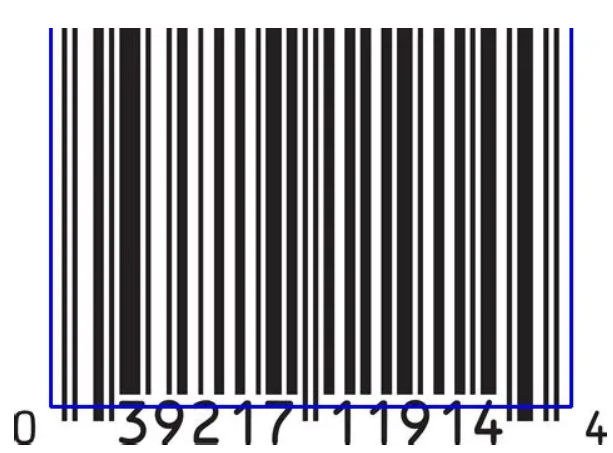
\includegraphics[width=\textwidth]{Pyzbar/BarcodeReader}
	\caption{Pyzbar - Barcode Reader}\label{Barcode Reader}
\end{figure}


\subsection{Handling QR Codes}
QR codes often contain embedded data such as URLs, contact information, or plain text. Follow these steps to extract data:
\begin{enumerate}
	\item Load the image containing the QR code.
	\item Use the \PYTHON{decode()} function from \texttt{pyzbar} to detect the QR code.
	\item Convert the \texttt{data} attribute from bytes to a readable string.
\end{enumerate}

\paragraph{Example Code:}
\begin{lstlisting}[language=Python]
	from pyzbar.pyzbar import decode
	from PIL import Image
	
	# Load the image with a QR code
	image = Image.open('qrcode_example.png')
	
	# Decode the QR code
	decoded_qr = decode(image)
	
	# Extract and print the data
	for qr in decoded_qr:
	print(f"Data: {qr.data.decode('utf-8')}")
	print(f"Type: {qr.type}")
\end{lstlisting}

\subsection{Multiple Barcode Detection}

The \PYTHON{decode()} function can handle multiple barcodes or QR codes in a single image. Each detected barcode is returned as an individual \texttt{Decoded} object in the result list.

\paragraph{Example Code:}
\begin{lstlisting}[language=Python]
	from pyzbar.pyzbar import decode
	from PIL import Image
	
	# Load the image with multiple barcodes
	image = Image.open('multiple_barcodes.png')
	
	# Decode all barcodes in the image
	decoded_objects = decode(image)
	
	# Print details of each detected barcode
	for index, obj in enumerate(decoded_objects):
	print(f"Barcode {index + 1}:")
	print(f"  Type: {obj.type}")
	print(f"  Data: {obj.data.decode('utf-8')}")
	print(f"  Bounding Box: {obj.rect}\n")
\end{lstlisting}

This script processes multiple barcodes in the image and prints their respective details.

\begin{figure}[h]
	\centering
	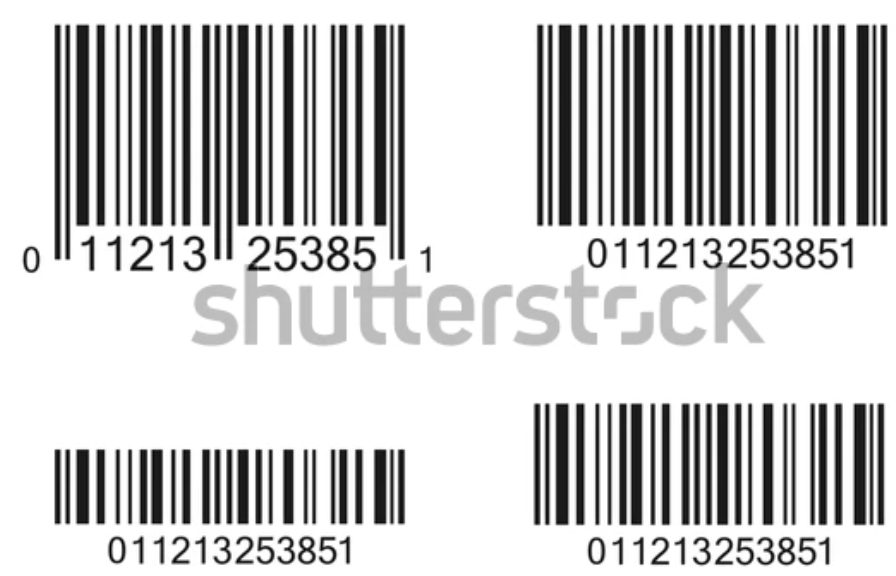
\includegraphics[width=\textwidth]{Pyzbar/MultipleBarcode}
	\caption{Pyzbar - Multiple barcodes in the image}\label{Multiple Barcode}
\end{figure}

\section{Example - Advanced Usage of Pyzbar}

Barcodes and QR codes are widely used for encoding data in compact formats, enabling quick data retrieval in industries like logistics, retail, and healthcare. Python libraries such as \texttt{pyzbar} and \texttt{zxing} offer tools to decode these codes programmatically. This report delves into customizing barcode decoding, managing specific barcode types, and processing multiple barcodes in a single image, catering to scenarios where default decoding mechanisms are insufficient.\cite{pyzbargithub:2024}\\

\subsection{Customizing Decoding}
Customizing barcode decoding allows developers to optimize performance for specific use cases. \texttt{pyzbar} provides flexibility to set parameters that suit particular barcode formats or environmental conditions.

\subsubsection{Adjusting Image Preprocessing}
Barcode decoding can be affected by image quality, such as lighting, contrast, or noise. Preprocessing techniques like binarization, resizing, and filtering can enhance accuracy. For instance, using the \texttt{Pillow} package for image preprocessing:
\begin{lstlisting}[language=Python]
	from PIL import Image, ImageEnhance
	from pyzbar.pyzbar import decode
	
	# Load and enhance the image
	image = Image.open('barcode_image.jpg')
	image = ImageEnhance.Contrast(image).enhance(2.0)
	
	# Decode the barcode
	decoded_objects = decode(image)
	for obj in decoded_objects:
	print(f"Type: {obj.type}, Data: {obj.data.decode('utf-8')}")
\end{lstlisting}
Enhancing contrast or converting the image to grayscale can significantly improve decoding accuracy.

\subsubsection{Restricting Decoding to Specific Barcode Types}

When working with a known barcode format, decoding performance can be optimized by restricting the detection to specific types. This reduces unnecessary computation and false positives:

\begin{lstlisting}[language=Python]
	from pyzbar.pyzbar import decode, ZBarSymbol
	
	# Restrict decoding to QR codes only
	decoded_objects = decode(image, symbols=[ZBarSymbol.QRCODE])
	for obj in decoded_objects:
	print(f"QR Code Data: {obj.data.decode('utf-8')}")
\end{lstlisting}
This approach is particularly useful when working in controlled environments, such as retail point-of-sale systems.

\subsection{Handling multiple barcodes in a single image}

In scenarios where multiple barcodes are present, it is crucial to decode all detectable barcodes efficiently. The \texttt{pyzbar} package supports multiple barcode decoding:
\begin{lstlisting}[language=Python]
	# Decode all barcodes in the image
	decoded_objects = decode(image)
	for obj in decoded_objects:
	print(f"Type: {obj.type}, Data: {obj.data.decode('utf-8')}")
\end{lstlisting}
Each decoded object contains metadata, such as the type of barcode and its data, which can be processed further.

\subsection{Working with specific barcode types.}

Different barcode types, such as EAN-13, Code 128, or QR codes, have unique structures and applications. Developers can tailor their decoding logic based on the barcode's specifications.

\subsubsection{Reading EAN-13 Codes}
EAN-13 barcodes are commonly used in retail for product identification. \texttt{pyzbar} decodes EAN-13 seamlessly:

\begin{lstlisting}[language=Python]
	# Decode EAN-13 barcodes
	decoded_objects = decode(image, symbols=[ZBarSymbol.EAN13])
	for obj in decoded_objects:
	print(f"EAN-13 Data: {obj.data.decode('utf-8')}")
\end{lstlisting}

Applications include inventory management and automated checkout systems.

\subsubsection{Reading QR Codes with Embedded Data}

QR codes can store diverse data types, such as URLs, text, or contact information. For QR code processing:
\begin{lstlisting}[language=Python]
	# Decode QR codes and extract data
	decoded_objects = decode(image, symbols=[ZBarSymbol.QRCODE])
	for obj in decoded_objects:
	print(f"QR Data: {obj.data.decode('utf-8')}")
\end{lstlisting}
QR codes are widely used in marketing campaigns and payment systems.\cite{Gs1:2024}

\section{Integration with Other Libraries}

Python's versatility is evident in its ability to integrate seamlessly with a wide range of libraries, enhancing its utility across diverse domains. Libraries such as \texttt{NumPy}, \texttt{Pandas}, and \texttt{Matplotlib} are frequently used together to perform advanced data analysis and visualization tasks. Similarly, libraries like \texttt{pyzbar} can integrate with image-processing tools such as \texttt{Pillow} to decode barcodes and QR codes efficiently. This modularity is facilitated by Python’s robust ecosystem, allowing developers to chain functionalities across libraries effortlessly. For instance, a decoded QR code from \texttt{pyzbar} can be directly processed using \texttt{Pandas} for data manipulation or stored in a database using \texttt{SQLAlchemy}. Such integration accelerates development and enables the creation of complex workflows with minimal overhead.\cite{pyzbarpypi:2024}\\

\section{Error Handling and Limitations}
While Python libraries offer extensive functionality, they are not without challenges. Error handling in libraries often requires developers to anticipate potential issues such as missing dependencies, unsupported formats, or runtime errors. For example, when using \texttt{pyzbar}, errors may occur if the ZBar package is not installed correctly on the host system. \cite{pyzbarpypi:2024} 

Additionally, limitations such as restricted support for certain barcode formats or degraded performance with low-resolution images can impact usability. To address these, libraries often provide comprehensive exception handling mechanisms. Developers are encouraged to use \texttt{try-except} blocks to gracefully manage runtime errors and log detailed information for debugging. However, the responsibility of understanding a package’s documented limitations lies with the user to ensure robust and reliable implementations.\cite{pyzbargithub:2024}


\section{Further Resources}

\textit{Barcode Detection Using OpenCV and Pyzbar} \cite{Utekarbarcode:2023}: 

This Medium article offers a hands-on tutorial on using \texttt{pyzbar} alongside OpenCV for barcode detection and decoding. It provides step-by-step instructions for integrating the two libraries, emphasizing how \texttt{pyzbar} can decode barcodes while OpenCV handles image preprocessing. The guide includes Python code examples, highlights common use cases such as QR code detection, and offers tips for optimizing barcode recognition in real-world scenarios. This resource is ideal for beginners and intermediate developers working on computer vision projects.

\textit{Detecting and Decoding Barcodes with Pyzbar} \cite{Techtutorialsx:2020}: 

This article delves into the functionality of the \texttt{pyzbar} package. It explains the installation process, basic usage, and how to decode barcodes from image files. The author also explores handling various barcode formats, offering practical code snippets to demonstrate these capabilities. The post addresses common issues, such as low-resolution image handling, making it an invaluable resource for developers implementing barcode scanning applications.

\textit{Pyzbar Official Documentation and Examples}  \cite{pyzbargithub:2024}: 

The official GitHub repository for \texttt{pyzbar} provides authoritative documentation, installation guidelines, and example usage. It includes detailed explanations of the package’s functionality, such as decoding QR codes and barcodes from images and camera feeds. The examples demonstrate the straightforward integration of \texttt{pyzbar} into Python projects, highlighting its versatility and ease of use. This is an essential reference for developers seeking to understand \texttt{pyzbar}'s full potential.

\textit{Pyzbar on PyPI} \cite{pyzbarpypi:2024}: 

The Python Package Index (PyPI) page for \texttt{pyzbar} is a foundational resource for understanding the package's scope. It provides installation instructions, dependency details, and compatibility information. Additionally, it includes a brief overview of the package’s features, such as its support for various barcode types, making it a starting point for developers exploring \texttt{pyzbar}.